\documentclass[a4paper]{article}

%%%%%%%%%%%%%%%%%%%%%%%%%%%%%%%%%%%%%%%%%%%%%%
\usepackage[T1]{fontenc}
\usepackage{geometry}
\geometry{a4paper,left=1.5cm,right=1cm,top=1cm,bottom=1cm}

\usepackage{graphicx}
\usepackage[absolute,overlay]{textpos}
\usepackage{eso-pic}               % image de fond
\usepackage{fontawesome5}
\usepackage[hidelinks]{hyperref}
\usepackage{tikz}
\usepackage{xcolor}
\usepackage{enumitem}
\setlist{nosep,leftmargin=6mm}
\usepackage{times}                % même police que votre exemple
\usepackage{array} 
\usepackage{tabularx}
\usepackage{ragged2e}
\let\origcolorbox\colorbox    % sauvegarde
\renewcommand{\colorbox}[2]{#2}% neutralise le fond
%%%%%%%%%%%%%%%%%%%%%%%%%%%%%%%%%%%%%%%%%%%%%%
%\definecolor{texcolor}{HTML}{e2e8f0}
\providecolor{sidetext}{rgb}{1,1,1}
\definecolor{maincolor}{HTML}{ffffff}

%%%%%%%%%%%%%%%%%%%%%%%%%%%%%%%%%%%%%%%%%
% — Ne changez pas le nom : « background.jpg » doit être présent
\AddToShipoutPictureBG*{%
  
\includegraphics[width=\paperwidth,height=\paperheight]{background.jpg}%
}

%%%%%%%%%%%%%%%%%%%%%%%%%%%%%%%%%%%%%%%%%
\newcommand{\fullrule}{\hspace{-1.5cm}\rule{\paperwidth}{0.4pt}}
\newcommand{\cvsection}[1]{%
  \vspace{6pt}\textbf{\Large #1}\par\vspace{2pt}}
\newcommand{\cicon}[1]{%
  \tikz[baseline]{\draw[fill=white] (0,0.1) circle[radius=0.1cm];}~#1}

\setlength{\parindent}{0pt}
%\color{texcolor}
%%%%%%%%%%%%%%%%%%%%%%%%%%%%%%%%%%%%%%%%%%%%%%%%%%%%%%%%%%%%%%
\begin{document}
\color{white}
% ---------- Photo ------------------------------------------------
\begin{textblock*}{4cm}(0.2cm,0.3cm)
  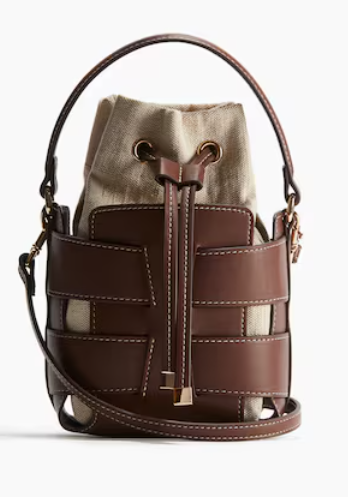
\includegraphics[width=2.5cm,clip,keepaspectratio]{aac821fb0ab3478982097188c59c68b7.png}
\end{textblock*}

% ---------- En-tête ---------------------------------------------
\begin{center}
  {\fontsize{44pt}{24pt}\selectfont\bfseries Judikael Mourouvin}

  \bigskip
  {\Large Technicien systèmes \& marketing digital}

  \bigskip\bigskip
  \faMapMarker~Route de COCOYER\ 97190 GOSIER
  \quad\faEnvelope~\href{mailto:jkmou971@gmail.com}{jkmou971@gmail.com}

  \bigskip
  % Badge LinkedIn (retirez-le si inutile)
  \faPhone~ +590 0690 91 14 48
  \quad \faLinkedin\ \href{}{}
 

  \vspace{-0.3cm}
  \fullrule
\end{center}

% ---------- Profil ----------------------------------------------
\cvsection{Profil}
Passionné par l’informatique et le marketing digital, je maîtrise la configuration de postes, la maintenance et le support aux utilisateurs. Mon année d’alternance à la DSI de la Mairie du Gosier m’a permis de piloter des projets numériques et d’affûter mes compétences en communication digitale. Désireux de poursuivre à temps plein, j’apporte rigueur, réactivité et sens du service pour mener à bien vos projets.

\medskip\fullrule

% ---------- Expérience ------------------------------------------
\cvsection{Expérience}
\hspace*{1.3cm}%

\colorbox{maincolor}{%
  \begin{minipage}{\linewidth}
    \textbf{Alternant en Marketing Digital} \\ Mairie du Gosier, DSI \\ 2023-2024
    \begin{itemize}
      \item Conduit divers projets numériques pour la mairie, garantissant leur déploiement selon le planning établi. \item Analysé les besoins des agents et implémenté des solutions digitales adaptées, optimisant les processus internes. \item Fournit support et formation aux utilisateurs tout en appuyant la stratégie de marketing digital de la collectivité.
    \end{itemize}
  \end{minipage}}

\vspace{3mm}


\colorbox{maincolor}{%
  \begin{minipage}{\linewidth}
    \textbf{Animateur de la zone informatique} \\ POLE EMPLOI, Gosier \\ 2022-2023
    \begin{itemize}
      \item Assuré l’assistance quotidienne des demandeurs et conseillers, résolvant rapidement leurs problèmes techniques. \item Installé, configuré et maintenu les postes de travail du site, garantissant leur disponibilité. \item Diagnostiqué les incidents matériels et logiciels, appliquant les correctifs pour minimiser les interruptions.
    \end{itemize}
  \end{minipage}}

\vspace{3mm}


\colorbox{maincolor}{%
  \begin{minipage}{\linewidth}
    \textbf{Stagiaire Informaticien} \\ NUMERIKA, Baie Mahault \\ 2020-2021
    \begin{itemize}
      \item Configuré et entretenu les équipements informatiques du parc, améliorant leur performance. \item Offert un support de proximité aux utilisateurs, facilitant l’utilisation des outils numériques. \item Participé à la maintenance préventive, réduisant les pannes récurrentes.
    \end{itemize}
  \end{minipage}}

\medskip\fullrule

% ---------- Éducation -------------------------------------------
\cvsection{Éducation}
\hspace*{1.3cm}%

    \begin{tabularx}{\linewidth}{@{}c >{\RaggedRight\arraybackslash}X@{}}
    \textcolor{sidetext}{\faGraduationCap} &
    \textbf{Bachelor Marketing Digital} \\
    & CFA IUTS \\
    & \textit{2023-2024} \\
    \end{tabularx}
    \begin{itemize}[leftmargin=*]
  \item Apprentissage des leviers SEO/SEA, réseaux sociaux et content marketing.
  \item Gestion de projets digitaux, analyse de données et mesure de performance.
  \item Conception de stratégies de communication en ligne alignées sur les objectifs business.
\end{itemize}
\vspace{3mm}

    \begin{tabularx}{\linewidth}{@{}c >{\RaggedRight\arraybackslash}X@{}}
    \textcolor{sidetext}{\faGraduationCap} &
    \textbf{BTS Système Numérique option Informatique et Réseaux} \\
    & Lycée de Chevalier Saint Georges, Abymes \\
    & \textit{2019-2021} \\
    \end{tabularx}
    \begin{itemize}[leftmargin=*]
  \item Étude des architectures systèmes et réseaux, protocoles et sécurité.
  \item Mise en œuvre de solutions d’administration, maintenance et support.
  \item Réalisation de projets techniques intégrant programmation et interconnexion d’équipements.
\end{itemize}

\medskip\fullrule

% ---------- Compétences -----------------------------------------
\cvsection{Compétences}

\hspace*{2.2cm}%
\begin{tabular}{@{}p{0.25\linewidth}p{0.18\linewidth}p{0.18\linewidth}p{0.18\linewidth}}\cicon Administration & \cicon Réseaux & \cicon Support & \cicon Maintenance \\
\cicon Marketing & \cicon Configuration & \cicon Diagnostic & \cicon Formation \\
\cicon Analyse & \cicon Gestion & ~ & ~ \\\end{tabular}   % grille 3 lignes × 4 colonnes

\end{document}
